\documentclass[UTF8]{ctexart}
\usepackage{geometry,amsmath,amssymb,theorem,caption,extarrows,mathrsfs,cite,citeref}
\usepackage{graphicx,xcolor,listings,geometry,booktabs,subfigure,tikz}
\usepackage{pgfplots,grffile}
\pgfplotsset{compat=newest}
  %% the following commands are needed for some matlab2tikz features
\usetikzlibrary{plotmarks}
\usetikzlibrary{arrows.meta}
\usetikzlibrary{calc}
\usepgfplotslibrary{patchplots}
\usepackage{xeCJK,fontspec}
\setCJKmainfont[BoldFont=方正小标宋简体,ItalicFont=楷体]{华文宋体}
  \setCJKsansfont{黑体}%serif是有衬线字体sans serif无衬线字体。
  %\setmonofont{CMU Typewriter Text} % 等寬字型
  \XeTeXlinebreaklocale "zh"
  \XeTeXlinebreakskip = 0pt plus 1pt minus 0.1pt
\lstset{
    basicstyle          =   \sffamily,          % 基本代码风格
    keywordstyle        =   \bfseries,          % 关键字风格
    commentstyle        =   \rmfamily\itshape,  % 注释的风格,斜体
    stringstyle         =   \ttfamily,  % 字符串风格
    flexiblecolumns,                % 别问为什么,加上这个
    numbers             =   left,   % 行号的位置在左边
    showspaces          =   false,  % 是否显示空格,显示了有点乱,所以不现实了
    numberstyle         =   \tiny\ttfamily,    % 行号的样式,小五号,tt等宽字体
    showstringspaces    =   false,
    captionpos          =   t,      % 这段代码的名字所呈现的位置,t指的是top上面
    frame               =   shadowbox,   % 显示边框
    rulesepcolor=\color{red!20!green!20!blue!20}
}

\lstdefinestyle{Python}{
    language        =   Python, % 语言选Python
    backgroundcolor=\color{backpycol},
    basicstyle      =   \tiny\ttfamily,
    numberstyle     =   \tiny\ttfamily,
    keywordstyle    =   \color{blue},
    keywordstyle    =   [2] \color{teal},
    stringstyle     =   \color{magenta},
    commentstyle    =   \color[HTML]{338AAF}\ttfamily,
    breaklines      =   true,   % 自动换行,建议不要写太长的行
    columns         =   fixed,  % 如果不加这一句,字间距就不固定,很丑,必须加
    basewidth       =   0.5em,
}
\definecolor{codegreen}{rgb}{0,0.6,0}
\definecolor{codegray}{rgb}{0.5,0.5,0.5}
\definecolor{codepurple}{rgb}{0.58,0,0.82}
\definecolor{backcolour}{rgb}{0.95,0.95,0.92}
\definecolor{backpycol}{rgb}{0.97,0.95,0.97}
\lstdefinestyle{C++}{
    language =[ANSI]C,
    backgroundcolor=\color{backcolour},
    commentstyle=\color[HTML]{338AAF}\ttfamily,
    keywordstyle=\tiny\sffamily\bfseries\color{magenta},
    numberstyle=\tiny\color{codegray},
    stringstyle=\color{codepurple},
    basicstyle=\tiny\ttfamily,
    breakatwhitespace=false,
    breaklines=true,
    basewidth=0.5em,
    captionpos=b,
    columns=fixed,
    frame=shadowbox,
    keepspaces=true,
    numbers=left,
    numbersep=5pt,
    showspaces=false,
    showstringspaces=false,
    showtabs=false,
    tabsize=4
}
\lstdefinestyle{matlab}{
    language=matlab,
    backgroundcolor=\color{backcolour},
    commentstyle=\color[HTML]{338AAF}\ttfamily,
    keywordstyle=\tiny\sffamily\bfseries\color{magenta},
    numberstyle=\tiny\color{codegray},
    stringstyle=\color{codepurple},
    basicstyle=\tiny\ttfamily,
    breakatwhitespace=false,
    breaklines=true,
    basewidth=0.5em,
    captionpos=b,
    columns=fixed,
    keepspaces=true,
    numbers=left,
    numbersep=5pt,
    showspaces=false,
    showstringspaces=false,
    showtabs=false,
    tabsize=4,
    frame=shadowbox
}
\definecolor{mygreen}{rgb}{0,0.6,0}
\definecolor{mygray}{rgb}{0.5,0.5,0.5}
\definecolor{mymauve}{rgb}{0.58,0,0.82}
\definecolor{bggray}{rgb}{0.93,0.95,0.94}
\lstdefinestyle{pseudocode}{
  backgroundcolor=\color{bggray},
columns=fullflexible,
tabsize=4,
breaklines=true,               % automatic line breaking only at whitespace
captionpos=b,                  % sets the caption-position to bottom
commentstyle=\color{mygreen},  % comment style
escapeinside={\%*}{*)},        % if you want to add LaTeX within your code
keywordstyle=\color{blue},     % keyword style
stringstyle=\color{mymauve}\ttfamily,  % string literal style
frame=shadowbox,
rulesepcolor=\color{red!20!green!20!blue!20},
% identifierstyle=\color{red},
language=c++,
numbers=left,
numberstyle=\tiny\color{codegray},
basicstyle=\tiny\ttfamily,% size of fonts used for the code
escapeinside=``,
xleftmargin=0.6em,
xrightmargin=0.6em,
aboveskip=1em
}
\newcommand{\dif}{\mathop{}\!\mathrm{d}}
\newcommand{\tr}{\mathop{}\!\mathrm{T}}
\newcommand{\const}{\mathop{}\!\mathrm{const.}}
%%%%%%%%%% Start TeXmacs macros
\catcode`\<=\active \def<{
\fontencoding{T1}\selectfont\symbol{60}\fontencoding{\encodingdefault}}
\catcode`\>=\active \def>{
\fontencoding{T1}\selectfont\symbol{62}\fontencoding{\encodingdefault}}
\newcommand{\barsuchthat}{|}
\newcommand{\divides}{\mathrel{|}}
\newcommand{\mathd}{\mathrm{d}}
\newcommand{\tmmathbf}[1]{\ensuremath{\boldsymbol{#1}}}
\newcommand{\tmop}[1]{\ensuremath{\operatorname{#1}}}
\newcommand{\tmtextbf}[1]{{\bfseries{#1}}}
\newcommand{\tmtextit}[1]{{\itshape{#1}}}
\newcommand{\splitline}{\noindent\rule[0.25\baselineskip]{\textwidth}{0.5pt}}
\newcommand{\autographinsert}[2]{\includegraphics[
  height=\dimexpr\pagegoal-\pagetotal-4\baselineskip\relax,width=#1\textwidth,
  keepaspectratio]{#2}}
  % NOTE: 插入图片如果出问题飘到下一页,请调整减掉的行数
\newtheorem{theorem}{定理}
%%%%%%%%%% End TeXmacs macros
\geometry{a4paper,left=1.8cm,right=1.8cm,top=1.5cm,bottom=1.5cm}
\begin{document}
\title{\textbf{Report for CS203B project}}
\author{** 作者 **}
\date{2020.11.16}
\maketitle
\tableofcontents

\section{Introduction}
\label{sec::Intro}
The multiplication of two matrices is one of the most basic operations of linear algebra and scientific computing. Modern signal processing, artificial intelligence and computer vision are all based on the fast and accurate algorithm of matrix multiplication, LU/QR/SVD decomposition and many other operations. For example, the FFT(Fast Fourier Transform) is based on the superior acceleration of the multiplication with FFT transforming matrices, and the CNN(Convolutional Neural Network) and many other NNs depend on the quick matrix operations boosted by the sophisticated algorithms and GPU/FPGA/etc. accelerators to achieve such a speed we've witnessed today.

\section{Background}
\label{sec::bgnd}

\section{Therotical Analysis}
\label{sec::TA}

The therotical analysis of all the algorithms and acceleration approaches we've taken in this project. From the brute-forcing approach of matrix multiplication, the Strassen's algorithm to the chache alignment and the BLAS \& LAPACK linear algebra library, the speed of matrix multiplication is increasing with the optimization goes from software, mathematics to engineering sophistication and specialized architectures.
\subsection{Brute-Force Algorithm}
\label{subsec::BFA}
Normal MM uses 3 nested loops to perform the vector dotting and traversal of the rows and columns of the 2 operands:
\begin{lstlisting}[language=matlab,style=pseudocode]
  STANDARD-MATRIX-MULTIPLY (A,B):
  let C be a new m*n matrix
    for i <- 1 to m
      for j <- 1 to n
        C[i,j] = 0
          for k = 1 to p
              C[i,j] += A[i,k]*B[k,j]
    return C
\end{lstlisting}
From the pseudocode above, let MUL, ADD, READ and WRITE refers the corresponding \(assembly\) commands of the computer.
Each nested loop multiplies the time complexity by its iteration number:
\begin{equation}
  \begin{aligned}
    T(\text{Naive})                  & =m\cdot n\cdot p\cdot (T(\text{\small MUL}+\text{\small ADD}+\text{\small READ}+\text{\small WRITE})) \\
                                     & =\Theta(mnp)                                                                                          \\
    m=n=p\Rightarrow T(\text{Naive}) & =\Theta(n^{3})
  \end{aligned}
\end{equation}

\subsection{Strassen Algorithm}
\label{subsec::STA}

Pseudocode of the Strassen algorithm:
\begin{lstlisting}[language=matlab,style=pseudocode]
    STRASSEN (MatrixA,MatrixB,Threshold)
        N=MatrixA.rows
      Let MatrixResult be a new N×N matrix
      if N<=Threshold
        MatrixResult=MatrixA*MatrixB // Recursion Point
      else
         // DIVIDE: partitioning input Matrices into 4 submatrices each
            for i  <-  0  to  N/2
              for j  <-  0  to  N/2
                  A11[i][j]  <-  MatrixA[i][j]
                  A12[i][j]  <-  MatrixA[i][j + N/2]
                  A21[i][j]  <-  MatrixA[i + N/2][j]
                  A22[i][j]  <-  MatrixA[i + N/2][j + N/2]

                  B11[i][j]  <-  MatrixB[i][j]
                  B12[i][j]  <-  MatrixB[i][j + N/2]
                  B21[i][j]  <-  MatrixB[i + N/2][j]
                  B22[i][j]  <-  MatrixB[i + N/2][j + N/2]
                  P1 <- STRASSEN(A11, B12-B22)          //P1=A11(B12-B22)
                  P2 <- STRASSEN(A11+A12, B22)          //P2=(A11+A12)B22
                  P3 <- STRASSEN(A21+A22, B11)          //P3=(A21+A22)B11
                  P4 <- STRASSEN(A22, B21-B11)          //P4=A22(B21-B11)
                  P5 <- STRASSEN(A11+A22, B11+B22)      //P5=(A11+A22)(B11+B22)
                  P6 <- STRASSEN(A12-A22, B21+B22)      //P6=(A12-A22)(B21+B22)
                  P7 <- STRASSEN(A11-A21, B11+B12)      //P7=(A11-A21)(B11+B12)

        // calculate the result submatrices
                  C11  <-  P5 + P4 - P2 + P6
                  C12  <-  P1 + P2
                  C21  <-  P3 + P4
                  C22  <-  P5 + P1 - P3 - P7

        // MERGE: put them together and make our resulting Matrix
                  for i  <-  0  to  N/2
                    for j  <-  0  to  N/2
                      MatrixResult[i][j]              <-  C11[i][j]
                      MatrixResult[i][j + N/2]        <-  C12[i][j]
                      MatrixResult[i + N/2][j]        <-  C21[i][j]
                      MatrixResult[i + N/2][j + N/2]  <-  C22[i][j]
                    end
                  end
              end
            end
        endif
      return MatrixResult
    endfunc
  \end{lstlisting}
Use the recursion function to evaluate the time complexity of the algorithm.
For \(n\geqslant 2\),
\begin{equation}
  \begin{aligned}
    T(2n)                          & =7T(n)+\Theta(n^{2})              \\
    \log_{2} n=k\Rightarrow T(k+1) & =7T(k)+\Theta(2^{2k})             \\
    \Rightarrow T(n)               & =O(n^{\log_{2}7})                 \\
                                   & \approx O(n^{2.81})<\Theta(n^{3})
  \end{aligned}
\end{equation}
The \(n\) in this result is the number of the \(Operation\), which is in propotition of the order of the matrix:
\begin{equation}
  t(n)=\alpha \text{Rows},\alpha\in(1,\infty)
\end{equation}
\subsection{Moreover on Algorithm-Only Optimizations}
\label{subsec::MoAOO}
The Strassen's algorithm opened a whole new possibility that the time complexity of matrix multiplication algorithm can be reduced to a degree less than 3. After the proposal of the Strassen's algorithm, there are a lot of its succesors like the Coppersmith-Winograd algorithm and the Harvard algorithm. These more sophisticated solutions are able to reduce the time complexity further, from the \(O(n^{2.81})\) record created by Strassen's algorithm to \(O(n^{2.373})\).
\subsection{Cache Alignement}
The fastest memory in the machine is the registers, and then the L1 cache, the slowest memory is the main RAM. Thus, the most time-comsuming step of the matrix multiplication program is reading data from the RAM into the registers, and the time cost can be significantly reduced by reducing the reading steps as many as possible. If the steps of reading data into the L3 caches from the RAM is minimized, and the remaining steps are only reading data from faster caches into the registers, the speed of the matrix multiplication is maximized. The discontinuous memory access is one of the main reasons for the slow computing speed of matrix multiplication.

The normal three nested for-loops follows the sequence of \(ijk\):

\begin{lstlisting}[style=pseudocode]
for i <- 1 to n
  for j <- 1 to n
    for k = 1 to n
      C[i,j] += A[i,k]*B[k,j]
\end{lstlisting}
For each element in C, the corresponding row of A and column of B are
multiplied and added in order. Since the matrix is stored by rows, the
total discontinuous "jumps" occur \(n^3+n^2-n\) times.Use the GCC compiler
to compile the C version of the naive multiplication, The assembly code of the naive solution
indicates this problem explicitly.

\begin{lstlisting}[style=pseudocode]
  .main:
    ...# LOOP
    ...# Initialize a[i][j]
    cltq
    ...# Initialize b[i][j]
    cltq
    ...# Initialize c[i][j]
    cltq
    movl	304(%rbp,%rax,4), %eax
    imull	%r8d, %eax
    leal	(%rcx,%rax), %edx
    movslq	%r9d, %rax
    movl	%edx, -96(%rbp,%rax,4)
    addl	$1, 1108(%rbp) # c[i][j]+=a[i][k]*b[k][j]
    ... #LOOP with unnecessary JMPs between the last element and the first element of a row
    movl	$0, %eax
    addq	$1248, %rsp
    popq	%rbp
    ret
  \end{lstlisting}

In order to accelerate algorithm, we change the sequence into \(ikj\):

\begin{lstlisting}[style=pseudocode]
  for i <- 1 to n
    for k <- 1 to n
      s=A[i,k]
      for j = 1 to n
          C[i,j] += s*B[k,j]
\end{lstlisting}

In this case, the total discontinuous "jumps" occur \(n^2\) times,
which is much less than the former case. Thus, the sequence of \(ikj\)
shall be a faster method. This inversion of the order in computing the
matrix multiplication has the maximized accuracy when accessing the
CPU cache, avoiding the interruption in the address sequence of the
processor. Use \lstinline{gcc -S} to generate the assembly code and analyze its structure:

\begin{lstlisting}[style=pseudocode]
  ... # entry of the program
  ... # Initialize a[i][k] and intermediate variable s
	cltq
	movl	704(%rbp,%rax,4), %eax
	movl	%eax, 1104(%rbp)
	movl	$0, 1108(%rbp) # s=a[i][k]
	jmp	.L4
.L5:
	... # Initialize c[i][j]
	cltq
	... # Initialize b[k][j]
	cltq
	movl	304(%rbp,%rax,4), %eax
	imull	1104(%rbp), %eax
	leal	(%rcx,%rax), %edx
	movslq	%r8d, %rax
	movl	%edx, -96(%rbp,%rax,4)
  addl	$1, 1108(%rbp) # C[i,j] += s*B[k,j]
  ... # loop and ret
\end{lstlisting}

\subsection{SIMD instructions and BLAS Library}
\label{subsec::SIMDIaBLASL}
The SIMD instructions can process a vector in a single clock cycle, by operating the data stored in special registers designed uniquely for performing SIMD operations.

A sample code using SIMD to accelerate the multiplication:

\begin{lstlisting}[language=C++,style=C++]
  template<int BM, int BK, int BN>
void sgemm_kernel(float *a, float *b, float *c) {
#define B_REG_M 2
//12
__m256 c_vec[B_REG_M*(BN/8)];

for(int i = 0; i < BM; i += B_REG_M) {
  for(int k = 0; k < B_REG_M*(BN/8); k++){
    c_vec[k] = _mm256_setzero_ps();
  }

  for(int k = 0; k < BK; k++) {
    __m256 b_vec[BN/8];
    for(int jj = 0; jj < BN/8; jj++){
      b_vec[jj] = _mm256_load_ps(b+k*BN+jj*8);// Use SIMD LOAD to load data into XMM registers
    }

    for(int ii = 0; ii < B_REG_M; ii++){
      __m256 a_vec = _mm256_broadcast_ss(a+(i+ii)*BK + k);// Use SIMD BROADCAST to broadcast data along with the internal bus

      for(int jj = 0; jj < BN/8; jj++) {//6
        __m256 temp = _mm256_mul_ps(a_vec, b_vec[jj]);
        c_vec[ii*(BN/8)+jj] = _mm256_add_ps(temp , c_vec[ii*(BN/8)+jj]);// SIMD add operation
      }
    }
  }

  for(int ii = 0; ii < B_REG_M; ii++){
    for(int jj = 0; jj < BN/8; jj++){
      _mm256_store_ps(c+(i+ii)*BN+jj*8, c_vec[ii*(BN/8)+jj]);// Store the data from XMM registers to RAM
    }
  }
}
#undef B_REG_M
}
\end{lstlisting}

\section{Methodology and Experiment Design}
\label{sec::ExpDesign}
In this section, we describe our specific implementation of our matrix
multiplication algorithm and the efforts to accelerate it as much as
possible.

In order to reduce unnecessary memory usage and save the running time,
we represent matrices by one-dimensional arrays, other than
two-dimensional. The relationship of the 1-D to 2-D conversion is: for 1D vector
\begin{equation}
  v={v_{1},\dots,v_{n^{2}}}
\end{equation}
and 2D matrix
\begin{equation}
  M=\left(
  \begin{matrix}
    m_{11} & m_{12} & \dots  & m_{1n} \\
    \vdots &        & \ddots & \vdots \\
    m_{n1} & m_{n2} & \dots  & m_{nn}
  \end{matrix}
  \right)
\end{equation}
There is a bijection \(T:V\leftrightarrow M\) for \(V:=\mathbb{R}^{n^{2}}\) and \(M:=\mathbb{R}^{n\times n}\), while \(r=n\) is the row size of the matrix:
\begin{equation}
  \forall v\in V,M_{ij}\in M,\mathrm{RMM}:V\leftrightarrow M:=M_{i+1j+1}=v_{n\times i+j}
\end{equation}
\(M_{ij}\)representing the item on row \(i+1\), column \(j+1\) of a
matrix by a 2-D array in C++ or Java,\(v_{i\times r+j}\) represents the same item in a 1-D
array, where n represents the total number of the columns. That is, the
matrix is stores by rows, or the matrix is stored by Row-Major.

We implement the algorithms using Java and C++ and used the corresponding Java and C++ code
to perform the benchmarking, and used Python in the data fitting process.

\subsection{Benchmark and Fitting code}
\label{subsec::BFC}

\paragraph{Benchmark code}~{}\\
\begin{lstlisting}[language=C++,style=C++]
  /**TEST CODE**/
    #include <...>
    int main(int argc, char *argv[]) {
      int turns = 10, rows = 2, cols = 2, interm = 0;
      randinit();
      for (int i = 0; i <= turns; i++) {
        LARGE_INTEGER t1, t2, tc;
        QueryPerformanceFrequency(&tc);
        QueryPerformanceCounter(&t1);
        /**Generate Rows and Elements**/
        printf_s("%3d   ", rows);
        /**Function To Be Timed**/
        QueryPerformanceCounter(&t2);
        time = (double) (t2.QuadPart - t1.QuadPart) / (double) tc.QuadPart;
        printf_s("%.3f\n", time);
        }
      getchar();
      return 0;
    }
\end{lstlisting}
\pagebreak
\paragraph{Python fitting code}~{}\\
\begin{lstlisting}[language=Python,style=python]
  import matplotlib.pyplot as plt
  import numpy as np
  from scipy.optimize import curve_fit

  x = np.array([
      # Matrix Size
  ])
  ynor = np.array([
      # MKL Results
  ])
  ystr = np.array([
    # Strassen Method Results
  ])


  def func(x, a, b, c):
  # y(x)=a*x^{b}+c
      return a * x**b + c

  popt1, pcov1 = curve_fit(func, x, ynor)
  popt2, pcov2 = curve_fit(func, x, ystr)

  ##
  Plotting functions
  ##
\end{lstlisting}

\subsection{Code implements of 11 experiments and optimizations}
The specific coding implementation of our experiment includes 11 parts:

\begin{enumerate}
  \def\labelenumi{\arabic{enumi}.}
  \item
        \textbf{the standard matrix multiplication (naive method/ brute-force
          method) for arbitrary size}

        As the pseudocode shows before, the standard matrix multiplication is
        computed by three nested for-loops.
  \item
        \textbf{extend brute-force method by partitioning matrices based on
          minimum alignment factor for arbitrary size}

        The minimum alignment factor means: factorizing the matrix order \(N\)
        into two factors such that the difference of the two factors is
        minimum.
  \item
        \textbf{normal Strassen's method (for matrix size of
          \(2^n \times 2^n\))}

        As the pseudocode shows before.
  \item
        \textbf{extend Strassen's method to arbitrary size, by padding zeros
          to the outermost so that the matrix size is \(2^n\times 2^n\)}
  \item
        \textbf{optimize Strassen's method by partitioning matrices based on
          factor of power-of-2 for even order matrices}
  \item
        \textbf{extend Strassen's method of \textless5\textgreater{} to
          arbitrary size, by padding zeros to the outermost so that the matrix
          size is \(2^n\times 2^n \)}
  \item
        \textbf{optimize Strassen's method of \textless4\textgreater{} by
          adding threshold judgment}

        According to our experimental test, we set the threshold as N=64. Once
        the size of submatrices is under 64 by 64, stop the Strassen's
        recursions and switch to the brute-force algorithm.
  \item
        \textbf{optimize Strassen's method of \textless6\textgreater{} by
          adding threshold judgment}
  \item
        \textbf{optimize Strassen's method of \textless8\textgreater{} by
          completing the matrix to make one factor be power-of-2}

        Other than padding zeros to the outermost to get \(2^n\times2^n\)
        matrices, we apply a cleverer way of matrix completion: padding
        appropriate zeros to make its size suitable for a good factorization
        which enables one factor to be a high-power-of-2.
  \item
        \textbf{optimize algorithm by exchanging the sequences of loops:
          change \(ijk\) into \(ikj\)}
  \item
        \textbf{implementation of \(MKL\) (Intel(R) Math Kernel Library)}

        The Intel(R) MKL is an optimized implementation of many math functions
        exclusively on x86 architecture and processors supports the Intel SIMD
        instructions, especially in Intel(R) processors. This library is
        implemented by assembly codes and C++ codes that are extremely
        optimized by Intel SIMD instructions (SSE,AVX), in order to maximize
        performance on matrix operations.
\end{enumerate}

The 11 parts above is a process of gradual optimization step by step for
the matrix multiplication algorithm. As a result of full investigation
and careful analysis, we eventually established our algorithm for
accelerating matrix multiplication.

In the experiment we use randomly generated square matrices of
increasing size with values in the range {[}-1,1{]} for test problems.

\section{Empirical Analysis}
\label{sec::EmpAnlys}
We split this experimental section. We present experimental results in
terms of the common method, algorithm optimization and hardware
optimization separately. Our experimental environment is:

CPU: Intel(R) Core(TM) i7-9750HQ@3.85 ̃4.05GHz

RAM: 32GB 2666MHz

\textbf{1. Naive method and Strassen's algorithm}

By implementing naive matrix multiplications and Strassen algorithm on
Java and fit the data, the standard data of the two algorithms are

\begin{equation}
  \begin{aligned}
    naive\ method                    & :\ \ \ T(N)=O(n^{3.371})   \\
    Strassen's\ (with\ threshold\ 2) & :\ \ \ T(S;2)=O(N^{3.546})
  \end{aligned}
\end{equation}

\begin{figure}[htb]
  \centering
  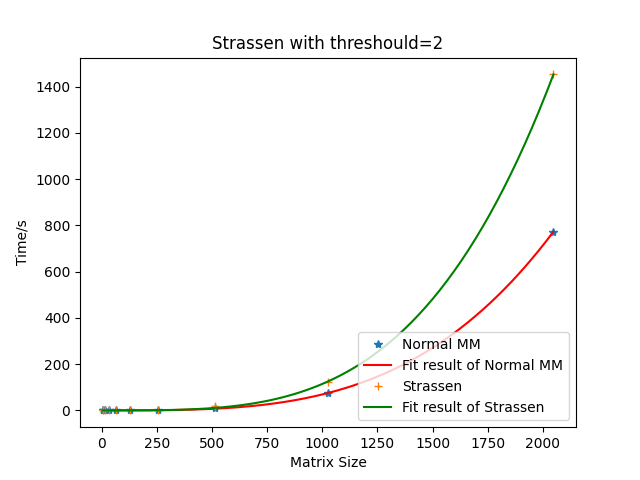
\includegraphics[height=7.0cm]{../ppt/slide-UIBK/th=2.png}
  \caption{}
\end{figure}

This result shows that the Strassen's Algorithm is seemingly faster than
the brute-force matrix multiplication, but neither of them even reaches
the time complexity of \(O(n^3)\).

\textbf{2. Strassen's algorithm with minimum size threshold}

The main reason causing the Strassen's algorithm slower than the
brute-forcing algorithm is the time costs in trace-backing the
recursion. Thus, the time cost of the Strassen's algorithm can be
significantly reduced by calibrating the crosspoint and setting the
minimum size of recursion.

\begin{equation}
  \begin{aligned}
    naive\ method                     & :\ \ \ T(N)=O(n^{3.384})    \\
    Strassen's\ (with\ threshold\ 32) & :\ \ \ T(S;32)=O(N^{3.337})
  \end{aligned}
\end{equation}

And the constant of the Strassen's algorithm is about 1/3 of that of the
brute-force algorithm.

\begin{figure}[htb]
  \centering
  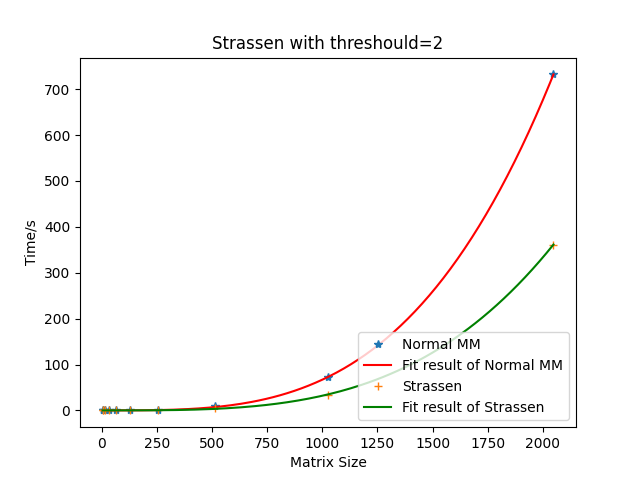
\includegraphics[height=7.0cm]{../ppt/slide-UIBK/th=64.png}
  \caption{}
\end{figure}

\textbf{3. Hardware optimization}

\textbf{(1) Cache alignment}

By implementing the \(ikj\) sequence of for-loops with improved cache
accuracy, as explained before, the Strassen's algorithm can meet the
theoretical time complexity:

\begin{equation}
  \begin{aligned}
    T(N)=O(n^{2.991}) \\
    T(S;32)=O(N^{2.816})
  \end{aligned}
\end{equation}

\begin{figure}[htb]
  \centering
  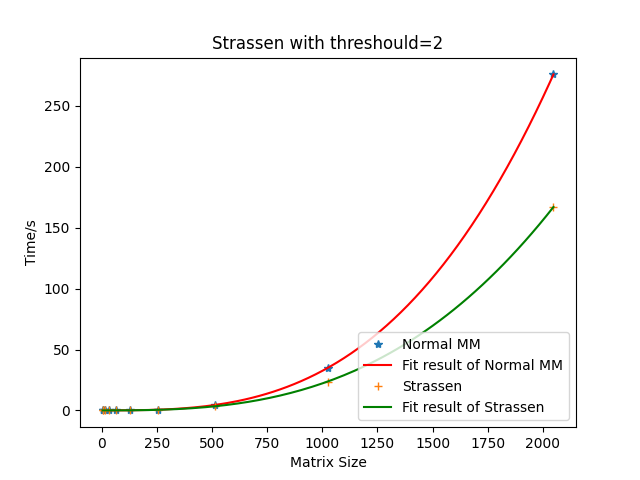
\includegraphics[height=6.8cm]{../ppt/slide-UIBK/th=32_ijk.png}
  \caption{}
\end{figure}

\begin{figure}[htb]
  \centering
  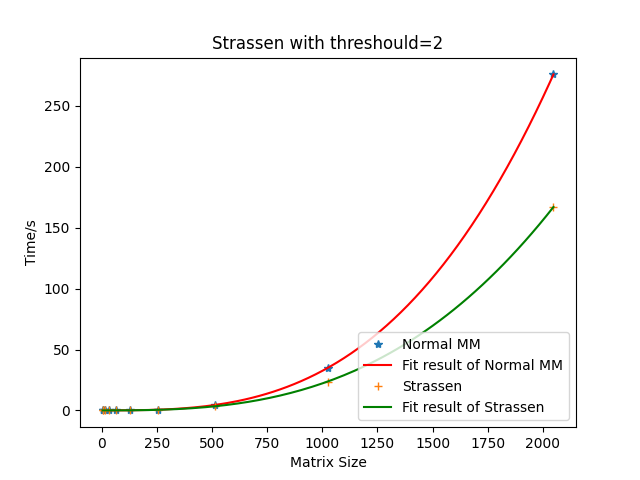
\includegraphics[height=7.0cm]{../ppt/slide-UIBK/th=64_ijk.png}
  \caption{}
\end{figure}

When the order of the matrix is very large, the length of the row-major
array may exceed the maximum capacity of the L1 cache, the speed of the
matrix multiplication will be limited. Thus, we implemented sectioned
matrix multiplication algorithm. Let s be the sectioning number which
the original matrix is divided by, and k be the polynomial degree of the
time complexity, divide the matrix into small chunks so that the length
of the chunks are below the maximum capacity of the L1 cache.

\begin{equation}
  \begin{aligned}
    T(n;s)                                          & =s^kt\left(\frac{n}{s}\right)^{k} \\
    \frac{n}{k} <  BW(L1\ Cache) \Rightarrow t(n/k) & =T(PUSH)+T(MUL)+T(TOP)            \\
                                                    & \ll 2T(MOV)+T(PUSH)+T(MUL)+T(TOP)
  \end{aligned}
\end{equation}

And we can get the time complexity by data fitting:

\begin{equation}
  \begin{aligned}
    T(N)   & =O(n^{3.013}) \\
    T(N;s) & =O(n^{2.822})
  \end{aligned}
\end{equation}

\begin{figure}[htb]
  \centering
  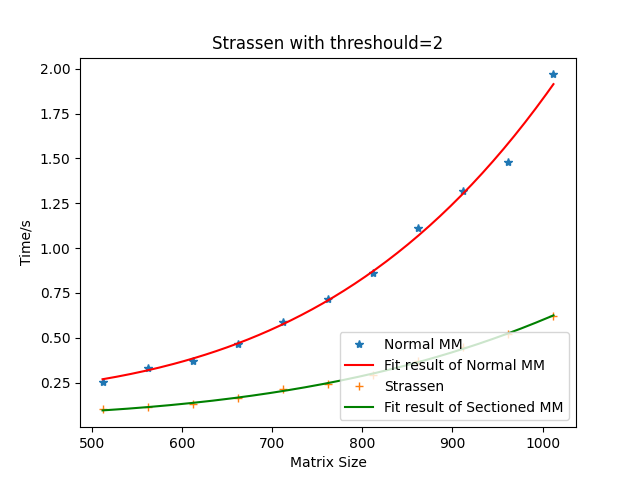
\includegraphics[height=6.7cm]{../ppt/slide-UIBK/sub_naive.png}
  \caption{}
\end{figure}

\textbf{(2) Implementation with Intel MKL}

Under the C++ implementation, the Intel MKL computes the 2500*2500
matrix multiplication within 6000 milliseconds, including filling the
arrays.

\begin{figure}[htb]
  \centering
  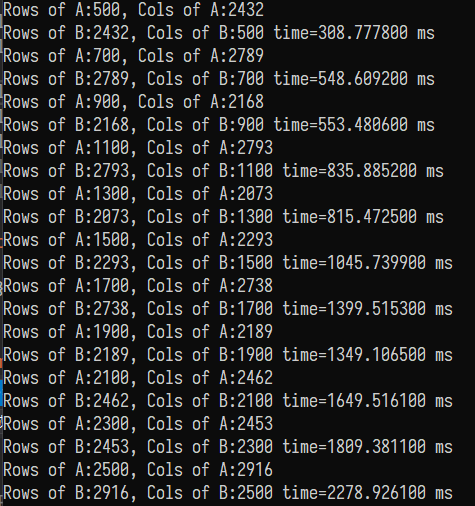
\includegraphics[height=7.0cm]{../ppt/slide-UIBK/mkl_dgemm.png}
  \caption{}
\end{figure}

Under the Java implementation, we adopted to accelerate the Strassen's
algorithm, the deletion of the unnecessary array filling progress
exploits the full capabilities of the MKL:

\begin{equation}
  \begin{aligned}
    T(N)   & =4.008\times 10^{-9}n^{3.052}\approx \frac{1}{f_{CPU}}n^{3.052}    \\
    T(MKL) & =1.817\times10^{-11}n^{2.982}\approx \frac{1}{250f_{CPU}}n^{2.982}
  \end{aligned}
\end{equation}

The extremely optimization based on the SIMD instructions of the Intel
CPU made the MKL run at 250x faster than the naive approach using merely
sequential operations.

\begin{figure}[htb]
  \centering
  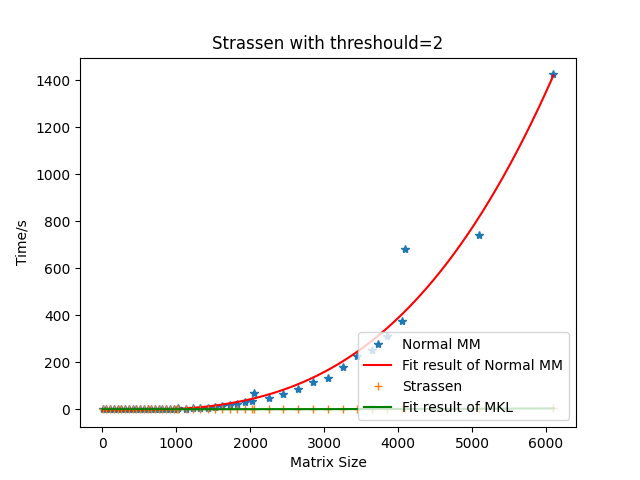
\includegraphics[height=6.3cm]{../ppt/slide-UIBK/mkl.png}
  \caption{}
\end{figure}
Now we have accelerated our matrix multiplication operation to a quite
optimal result.

\section{Conclusion}
\label{sec::Conc}

The earliest matrix multiplication optimisation algorithm is Strassen's algorithm\cite{strassen1969gaussian}, which was proposed by the German mathematician Volker Strassen in 1969 and bears his name. The algorithm is a classic and can be found in most textbooks on algorithms and computational optimisation. A basic introduction to the algorithm can also be found here. The main idea is to piece together some indirect terms and use the addition and subtraction of these indirect terms to eliminate some of the terms to get the final answer. In simple terms, it is addition and subtraction instead of multiplication. For a square matrix of order two, the multiplication operation, which would have taken 8\((=2^{3})\) times, is reduced to 7\((=2^{\log_{2} 7})\) times. The importance of this algorithm is twofold, firstly it reduces the time complexity of matrix multiplication, from \(O(n^3)\) to \(O(n^{\log_{2} 7})\),\(\log_{2} 7\) to approximately 2.807355. i.e. the original cubic operation is reduced in dimension (\(O(n^{2.807355})\)), however more importantly, this algorithm made mathematicians realise that this problem is not simply a three dimensional problem, but most likely lower dimensional problem, i.e., there may be a large scope for optimisation.

Since then, better algorithms have been proposed: Pan's algorithm\cite{pan1981new} in 1981 (\(O(n^{2.494})\)), the Coppersmith-Winograd algorithm\cite{COPPERSMITH1990251} in 1987 ((\(O(n^{2.376})\)), and an improved version of this algorithm published in 1990 (\(O(n^{2.3754})\)). After 1990, related research went into a 20-year-long hibernation period. It was only in 2010 that Andrew Stothers, a PhD student in the Department of Mathematics at the University of Edinburgh, proposed a new algorithm\cite{HARVEY20181} that further reduced the time complexity (\(O(n^{2.274})\)) in his PhD thesis, but he did not publish this result in journals or academic conferences himself! In late 2011, Virginia Vassilevska Williams at Stanford University reduced the time complexity\cite{article} to (\(O(n^{2.3731})\)), based on Andrew Stothers' work. The most optimised solution\cite{1401.7714} to date is the Stanford method, simplified by François Le Gall in autumn 2014, which achieves a time complexity of (\(O(n^{2.373})\)).

Throughout these decades, every bit of optimisation can be hard won and increasingly difficult, and it is fair to say that if one can now reduce the dimensionality by a difficult 0.0000001, it is a remarkable academic achievement. While searching for the optimal solution, a question naturally comes to the researchers' attention: what is the time complexity of the optimal solution of the matrix multiplication method? Is it possible to prove the time complexity of this optimal solution from a mathematical theory perspective? Even if we do not know the exact approach to the optimal solution for the time being? In other words, what is the true dimension of the problem. If we assume that the true dimension is D and the dimension of the brute-force solution is 3,then it follows naturally that
\begin{equation}
  2\leqslant T\leqslant 3
\end{equation}
Since the best algorithms are now reduced its degree of time complexity to 2.3728642, and a complete single access (writing the answer) for a square matrix of order N requires an operation of the order of 2 in N, we can further shrink the range:
\begin{equation}
  2< T\leqslant T_{\text{opt}}=2.373
\end{equation}

Based on all the data we've obtained above, we can plot the degree of all the optimized algorithms along with the time of their publication.
\begin{figure}[htb]
  \begin{center}
    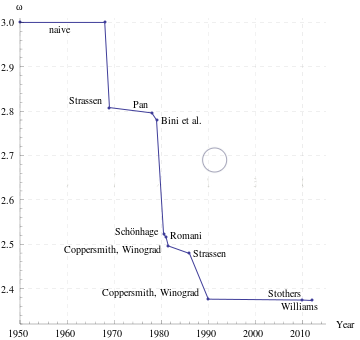
\includegraphics[height=6.3cm]{tend.png}
    \caption{Actual optimization achievement}
  \end{center}
\end{figure}
Then we're able to make a fitting to guess the minimum time complexity of the matrix multiplication. Use the Boltzmann double-exponential function
\begin{equation}
  \hat{D}(t)=\frac{A_{1}-A_{2}}{1+e^{(x-x_{0})/p}}+A_{2}
\end{equation}
to perform the fit:
\begin{figure}[htb]
  \begin{center}
    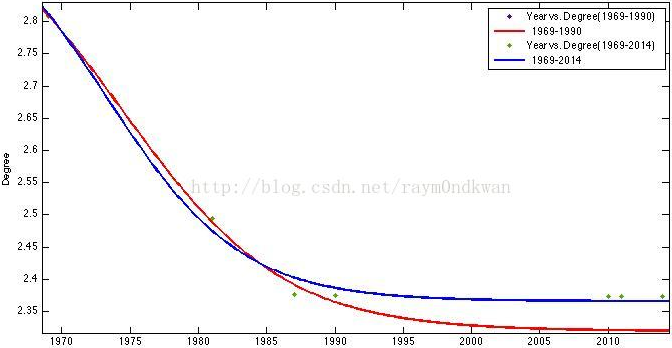
\includegraphics[height=6.3cm]{tend-fit.png}
    \caption{Fitted Optimization Tendency}
  \end{center}
\end{figure}

However, the algorithm algorhithm can only shrink the degree on the right corner of the \(n\) and the constant coefficient also play a very important role in reducing the total time complexity. Simply speaking, the constant coefficient is uniquely determined by the architecture of the computational system we adopted. The CPU is powerful in general tasks but the hardware structure of CPUs are hardly optimized in allusion to computation-dense tasks like matrix multiplication, so the CPUs have no outstanding performance in matrix multiplication we've been testing in this project. On the contrary, many other hardwares are designed optimally for high-speed matrix operations, for example the GPUs and FPGA chips. Using such highly aimed architectures with parallelized codes generated by special compilers can accelerate the speed of computation to a terrifying level:
\begin{figure}[htb]
  \begin{center}
    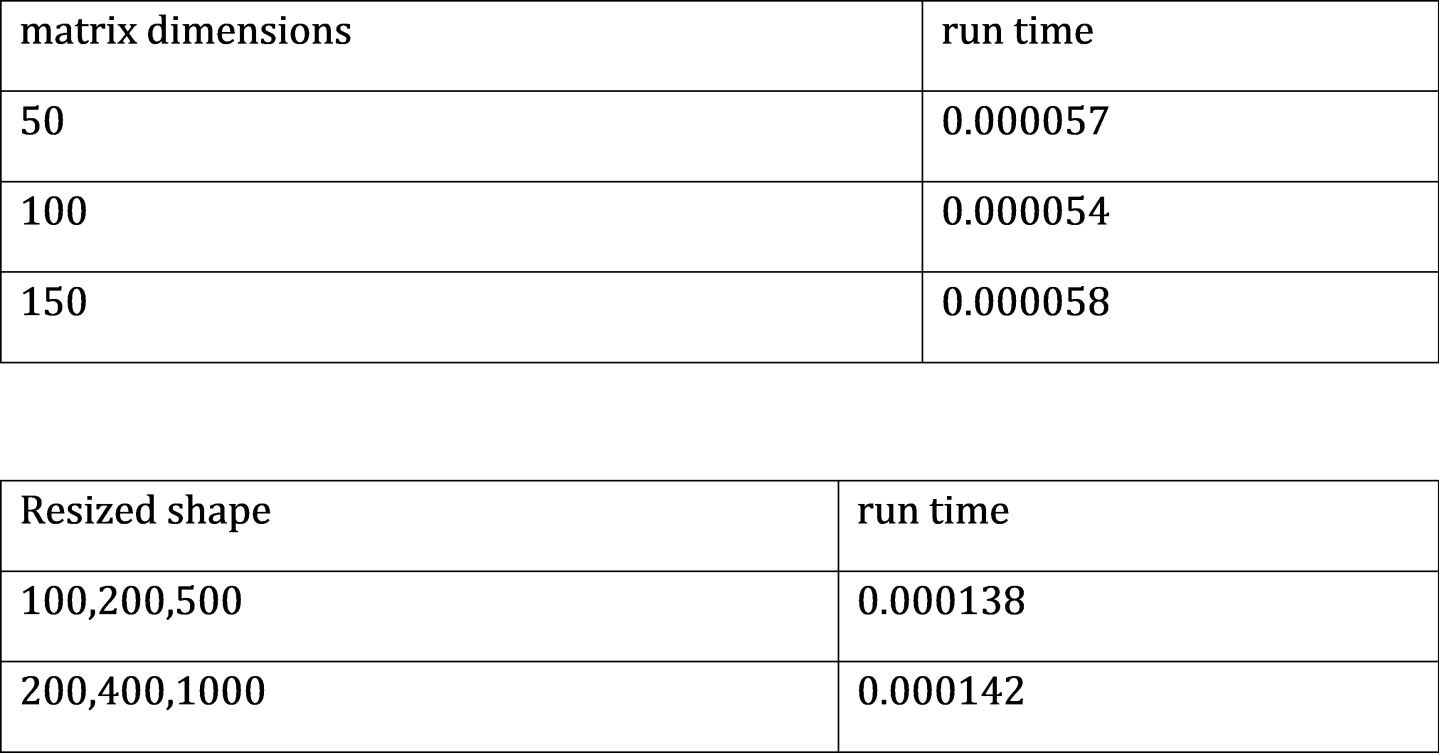
\includegraphics[height=6.3cm]{gpu_speed.jpg}
    \caption{Matrix Multiplication Benchmark Using GPU}
  \end{center}
\end{figure}

\bibliographystyle{ieeetr}
\bibliography{reference}
\end{document}